\documentclass[10pt]{beamer}

\input{/Users/daniel/Documents/LaTeX/beamer-style.tex}

\title{SGBD - 2\textsuperscript{e}}
\subtitle{Chapitre 5 - Transactions et accès concurrents Langage de Contrôle des données (LCD)}
\date{\today}
\author{Daniel Schreurs}
\institute{Haute École de la Province de Liège}
%\titlegraphic{\hfill\includegraphics[height=1.5cm]{logo.eps}}

\setbeamertemplate{frame footer}{\insertsectionhead}

\begin{document}

\maketitle

\setbeamerfont{subsection in toc}{size=\small}
\setbeamerfont{subsubsection in toc}{size=\normalsize}
\setbeamertemplate{section in toc}[sections numbered]
\setbeamertemplate{subsection in toc}[subsections numbered]
\setbeamertemplate{subsubsection in toc}[subsubsections numbered]
\begin{frame}[allowframebreaks]{Table des matières du chapitre}
    \tableofcontents[subsectionstyle=show/show/hide,subsubsectionstyle=show/show/hide,]
\end{frame}

\section{Introduction}
\tocss
\subsection{Définition}
\begin{frame}{\secname : \subsecname}
    Problèmes qui peuvent survenir lors de l'exploitation d'une base de données :
    \begin{itemize}
        \item Deux utilisateurs tentent de modifier la même donnée au même moment
        \item Une panne se produit pendant l'exécution d'une transaction
    \end{itemize}
\end{frame}

\begin{frame}{\secname : \subsecname}
    Ces deux problèmes sont résolus grâce au concept de transaction.
    \metroset{block=fill}
    \begin{alertblock}{Important}
        Une transaction est une unité de traitement cohérent et sûr.
    \end{alertblock}
    Toute requête doit être exécutée dans le contexte d'une transaction.
\end{frame}
\section{Notions de base}
\tocss
\subsection{Définition}
\begin{frame}{\secname : \subsecname}
    \metroset{block=fill}
    \begin{alertblock}{Important}
        Une base de données est dans un état cohérent si les valeurs contenues dans la base vérifient toutes les contraintes d'intégrité définies sur la base.
    \end{alertblock}
    Les transactions de mise à jour font passer la base d'un état à un autre.
    Une \textbf{transaction est cohérente} si elle fait passer la base d'un état cohérent à un autre état cohérent.
    Cependant, lors des mises à jour par des transactions cohérentes, la base peut passer par des \textbf{états intermédiaires incohérents}.
\end{frame}
\subsection{Exemple}
\begin{frame}{\secname : \subsecname}
    \lstinputlisting[language=plsql,title=Exemple]{../exemples/Chapitre 5/notion_de_base-exemple--1.sql}\footnote{Si on a une panne entre les 2 updates, on ne veut pas perdre le montant $S$. Et donc les 2 opérations doivent obligatoirement être réalisées toutes les deux ou aucune.}
\end{frame}
\subsection{Définition}
\begin{frame}{\secname : \subsecname}
    Une transaction peut-être constituée d'un ensemble d'actions.  Les actions sont des unités de traitement indivisibles.
    Une des grandes propriétés des transactions est l'\textbf{atomicité}.
    \metroset{block=fill}
    \begin{alertblock}{Important}
        Le terme \textbf{atomicité} signifie qu'une transaction doit être traitée comme une seule opération.
        Autrement dit, le gestionnaire des transactions doit assurer que toutes les actions de la transaction sont exécutées, ou bien qu'aucune ne l'est.
    \end{alertblock}
\end{frame}

\begin{frame}{\secname : \subsecname}
    Si l'exécution d'une transaction est interrompue à cause d'une panne, le SGBD doit être capable de décider des actions à entreprendre après la réparation.
    Il peut :
    \begin{itemize}
        \item \textbf{Compléter} la transaction en exécutant les actions restantes
        \item \textbf{Défaire} les actions qui avaient été exécutées avant la panne
    \end{itemize}
\end{frame}

\begin{frame}{\secname : \subsecname}
    Pour permettre au SGBD d'assurer l'atomicité des transactions, nous devons définir les actions qui indiquent le début et la fin d'une transaction.
    Le début d'une transaction indique au SGBD de démarrer une nouvelle transaction.
    Une transaction peut se terminer par l'action \textbf{valider ou annuler} dont les effets sur la base sont évidemment opposés.
\end{frame}

\begin{frame}{\secname : \subsecname}
    Trois issues sont possibles pour une transaction :
    \begin{itemize}
        \item Une vie sans histoire;
        \item Un arrêt interne;
        \item Un arrêt externe.
    \end{itemize}
\end{frame}
\subsection{Une vie sans histoire}
\begin{frame}{\secname : \subsecname}
    La transaction $T$ effectue successivement toutes ses actions lire et/ou écrire et exécute l'action valider.
    \textbf{$T$ a atteint son point de confirmation}.  Il s'agit d'un point de non-retour à partir duquel toutes les modifications faites sur la base par $T$ sont considérées comme irrémédiablement faites.
\end{frame}

\begin{frame}{\secname : \subsecname}
    La \textbf{durabilité} rend permanents les changements. Considérant aussi les pannes.
    La commande SQL qui valide et termine une transaction est : \lstinline[language=plsql]!COMMIT!
\end{frame}

\subsection{Un arrêt interne}
\begin{frame}{\secname : \subsecname}
    Exemple : lors de son exécution, une transaction \textbf{détecte une erreur} de conversion de type de données ou une violation de contrainte d'intégrité.
    Dans ce cas, la transaction arrête son exécution en émettant l'\textbf{action annuler}.
    Afin d'assurer la propriété d'atomicité, le SGBD doit effacer toute trace du passage de la transaction annulée.
    La commande SQL qui défait et termine une transaction est : \lstinline[language=plsql]!ROLLBACK!
\end{frame}

\subsection{Un arrêt externe}
\begin{frame}{\secname : \subsecname}
    Un événement extérieur vient arrêter définitivement l'exécution de la transaction.  Exemples :
    \begin{itemize}
        \item Action de l'utilisateur qui décide d'interrompre la transaction
        \item Action du SGBD qui a détecté un inter-blocage et qui, pour résoudre le problème, a choisi notre transaction comme victime
        \item Panne
    \end{itemize}
    Le SGBD doit effacer toute trace du passage de la transaction.
    Si l'arrêt a été provoqué par une panne, effacer les traces du passage de la transaction ne peut être réalisé qu'après le redémarrage du système : mécanisme (ou processus) de \textbf{reprise après panne} ou \textbf{recovery}.
\end{frame}
\begin{frame}{\secname : \subsecname}
    Le rôle du mécanisme de reprise après panne est double :
    \begin{itemize}
        \item Il doit assurer que les effets d'une transaction validée apparaîtront dans la base après la reprise
        \item Il doit assurer que les effets d'une transaction annulée n'apparaîtront pas dans la base après la panne
    \end{itemize}
\end{frame}
\section{Transactions concurrentes}
\tocss
\subsection{Définition}
\begin{frame}{\secname : \subsecname}
    Si des transactions cohérentes sont exécutées séquentiellement, elles conduisent toujours à un état final cohérent.
    Pour des raisons d'efficacité, il est nécessaire d'autoriser l'exécution concurrente des transactions.
    \metroset{block=fill}
    \begin{alertblock}{Important}
        On dit que deux transactions sont concurrentes si elles accèdent en même temps aux mêmes données.
    \end{alertblock}
    Il faut gérer ces exécutions concurrentes de manière à ce qu'elles ne conduisent pas à une base incohérente
\end{frame}

\begin{frame}{\secname : \subsecname}
    Les différentes transactions sont constituées d'actions lire et écrire et, si aucun mécanisme de contrôle de l'exécution n'est présent dans le SGBD, nous pouvons avoir les \textbf{3 types d'anomalies}:
    \begin{itemize}
        \item Pertes de mise à jour
        \item Lecture impropre
        \item Lecture non reproductible
    \end{itemize}
\end{frame}
\subsection{Pertes de mise à jour}
\begin{frame}{\secname : \subsecname}
    Soit les 2 transactions suivantes :
    \begin{table}[]
        \begin{tabular}{ll}
            T1 :  $Lire (x)$               & T2 :  $Lire (x)$               \\
            T1 : $x \longleftarrow x + 10$ & T2 : $x \longleftarrow x + 20$ \\
            T1 : $\acute{e}crire (x)$      & T2 : $\acute{e}crire (x)$
        \end{tabular}
    \end{table}
    Si exécutées séquentiellement, si x vaut 50 au départ, après l'exécution des deux transactions, x vaudra 80.
\end{frame}

\begin{frame}{\secname : \subsecname}
    Si exécutées de manière concurrente, nous pourrions avoir la séquence suivante :
    \begin{table}[]
        \begin{tabular}{ll}
            T1 :  $Lire (x)$               & (T1 lit 50 pour x)       \\
            T1 : $x \longleftarrow x + 10$ &                          \\
            T2 : $Lire (x)$                & (T2 lit 50 pour x)       \\
            T1 : $\acute{e}crire (x)$      & (dans la base x vaut 60) \\
            T2 : $x \longleftarrow x + 20$ &                          \\
            T2 : $\acute{e}crire (x)$      & (dans la base x vaut 70)
        \end{tabular}
        \caption*{Dans cet exemple, la mise à jour effectuée par $T1$ a été écrasée par celle faite par $T2$.}
    \end{table}
\end{frame}
\subsection{Lecture impropre}
\begin{frame}{\secname : \subsecname}
    \begin{table}[]
        \begin{tabular}{ll}
            T1                                                                                                            & T2                                                                                                     \\
            DÉBUT TRANSACTION                                                                                             & DÉBUT TRANSACTiON                                                                                      \\
            \begin{tabular}[c]{@{}l@{}}UPDATE comptes\\ SET solde = 25000\\ WHERE\\  num\_compte\\  = '007';\end{tabular} &                                                                                                        \\
                                                                                                                          & \begin{tabular}[c]{@{}l@{}}SELECT solde \\ FROM comptes\\ WHERE\\ num\_compte\\  = '007';\end{tabular} \\
            ROLLBACK;                                                                                                     &
        \end{tabular}
        \caption{Anomalie 2 : Lecture impropre}
    \end{table}
\end{frame}

\begin{frame}{\secname : \subsecname}
    \begin{itemize}
        \item À cause de la propriété d'atomicité, tout doit se passer comme si T1 n'avait jamais fait la modification dans la table comptes.
        \item La valeur lue par T2 est incorrecte, elle est impropre : T2 lit des données non confirmées !  Les données sont salies par T1.
        \item Effet domino : l'annulation de la transaction T1 doit entraîner l'annulation de toutes les transactions ayant lu des résultats intermédiaires de T1.
    \end{itemize}
\end{frame}

\begin{frame}{\secname : \subsecname}
    \begin{table}[]
        \begin{tabular}{ll}
            T1                                                                                                              & T2                                                                                                                \\
            DÉBUT TRANSACTION                                                                                               & DÉBUT TRANSACTiON                                                                                                 \\
            \begin{tabular}[c]{@{}l@{}}UPDATE comptes\\ SET solde = 25000\\ WHERE num\_compte= '007';\end{tabular}          &                                                                                                                   \\
                                                                                                                            & \begin{tabular}[c]{@{}l@{}}SELECT SUM(solde)\\ FROM comptes\\ WHERE\\ num\_compte IN ('007', '163');\end{tabular} \\
            \begin{tabular}[c]{@{}l@{}}UPDATE comptes\\ SET solde = solde + 200\\ WHERE\\ Num\_compte = '163';\end{tabular} &                                                                                                                   \\
            COMMIT;                                                                                                         &
        \end{tabular}
        \caption{Anomalie 2 : Lecture impropre sans annulation}
    \end{table}
\end{frame}

\begin{frame}{\secname : \subsecname}
    T2 puise ses valeurs dans la base alors qu'elle est dans un état intermédiaire incohérent.
\end{frame}

\begin{frame}{\secname : \subsecname}
    \begin{itemize}
        \item Anomalie 2 : Lecture impropre : \textbf{lecture ou référence fantôme}
        \item Une lecture ou référence fantôme \textbf{peut découler d'une lecture impropre}.
    \end{itemize}
\end{frame}

\begin{frame}{\secname : \subsecname}
    \begin{table}[]
        \begin{tabular}{ll}
            T1                                                                                & T2                                                                                          \\
            DÉBUT TRANSACTION                                                                 & DÉBUT TRANSACTiON                                                                           \\
            \begin{tabular}[c]{@{}l@{}}SELECT *\\ FROM eleves\\ WHERE annee = 2;\end{tabular} &                                                                                             \\
                                                                                              & \begin{tabular}[c]{@{}l@{}}INSERT INTO eleves\\ VALUES (11, 'Bloche', ..., 2);\end{tabular} \\
                                                                                              & COMMIT                                                                                      \\
            \begin{tabular}[c]{@{}l@{}}SELECT *\\ FROM eleves\\ WHERE annee = 2;\end{tabular} &
        \end{tabular}
        \caption{Anomalie 2 : Lecture impropre : lecture ou référence fantôme}
    \end{table}
\end{frame}

\begin{frame}{\secname : \subsecname}
    La transaction \textbf{T1 ne retrouve pas le même ensemble de tuples lors de la deuxième lecture} : un tuple supplémentaire apparaît.
    Il s'agit d'un \textbf{tuple fantôme}.
\end{frame}

\begin{frame}{\secname : \subsecname}
    \begin{table}[]
        \begin{tabular}{ll}
            T1                                                                                                                 & T2                                                                                                                                  \\
            DEBUT TRANSACTION                                                                                                  & DEBUT TRANSACTiON                                                                                                                   \\
            \begin{tabular}[c]{@{}l@{}}SELECT points\\ FROM resultats WHERE \\ num\_cours = 5 AND num\_eleve = 7;\end{tabular} &                                                                                                                                     \\
                                                                                                                               & \begin{tabular}[c]{@{}l@{}}UPDATE resultats\\ SET points = points * 1.10\\ WHERE num\_cours = 5 \\ AND num\_eleve = 7;\end{tabular} \\
                                                                                                                               & COMMIT                                                                                                                              \\
            \begin{tabular}[c]{@{}l@{}}SELECT points\\ FROM resultats WHERE\\ num\_cours = 5 AND num\_eleve = 7;\end{tabular}  &                                                                                                                                     \\
            COMMIT;                                                                                                            &
        \end{tabular}
        \caption{Anomalie 2 : Lecture non reproductible}
    \end{table}
\end{frame}

\begin{frame}{\secname : \subsecname}
    Remarques :
    \begin{itemize}
        \item \textbf{Lecture non reproductible} : On ré-exécute une requête et le résultat ne donne pas les mêmes valeurs que lors de la première exécution.
        \item \textbf{Référence fantôme} : On ré-exécute une même requête et le résultat donne une ligne supplémentaire par rapport à la première exécution
    \end{itemize}
    Dans les deux cas, les données ont été modifiées par une autre transaction !
\end{frame}

\subsection{ACID}
\begin{frame}{\secname : \subsecname}
    Jusqu'à présent, nous avons vu 3 propriétés des transactions :
    \begin{itemize}
        \item A	comme Atomicité
        \item C	comme Cohérence
        \item ?	comme ?
        \item D	comme Durabilité
    \end{itemize}
    Nous allons pouvoir ajouter \textbf{I} comme \textbf{ISOLATION}
\end{frame}

\subsection{isolation}
\begin{frame}{\secname : \subsecname}
    \metroset{block=fill}
    \begin{alertblock}{Important}
        L'isolation est la propriété des transactions qui exige que chaque transaction perçoive à tout instant la base dans un état cohérent.
        En d'autres termes, une transaction en cours d'exécution ne peut pas dévoiler ses effets aux autres transactions concurrentes avant d'atteindre son point de confirmation.
    \end{alertblock}
\end{frame}

\begin{frame}{\secname : \subsecname}
    La norme SQL2 distingue deux types de verrous
    \begin{itemize}
        \item Verrous courts : niveau instruction
        \item Verrous long : niveau transaction
    \end{itemize}
    Permet de résoudre :
    \begin{itemize}
        \item Perte de mise à jour
        \item Lecture impropre
        \item Lecture non reproductible
    \end{itemize}
\end{frame}

\begin{frame}{\secname : \subsecname}
    \metroset{block=fill}
    \begin{alertblock}{Important}
        4 niveaux d'isolation standardisés par SQL2 (Set Transaction Isolation Level):
        \begin{itemize}
            \item Degré 0 : READ UNCOMMITTED
            \item Degré 1 : READ COMMITTED
            \item Degré 2 : REPEATABLE READ
            \item Degré 3 : SERIALIZABLE
        \end{itemize}
    \end{alertblock}
\end{frame}

\begin{frame}{\secname : \subsecname}
    Isolation degré 0 : READ UNCOMMITTED
    \begin{itemize}
        \item Verrou court exclusif en écriture
        \item Verrou exclusif libéré après l'écriture
        \item Pas de pose de verrous lors des lectures
    \end{itemize}
    Permet d'éviter les pertes de mises à jour.
\end{frame}

\begin{frame}{\secname : \subsecname}
    Isolation degré 0 : \textbf{READ UNCOMMITTED} \\
    Verrou court exclusif écriture
    \begin{table}[]
        \begin{tabular}{ll}
            Transaction 1                                                                                               & Transaction 2                                                                                                                                                                                                                 \\
            \textbf{Verrou court exclusif écriture}                                                                     &                                                                                                                                                                                                                               \\
            \begin{tabular}[c]{@{}l@{}}UPDATE employes\\ SET bareme = bareme +10\\ WHERE numsecu = '1234';\end{tabular} & \begin{tabular}[c]{@{}l@{}}pas possibilité de MAJ du nr 1234,\\ tant que l’instruction UPD transaction 1\\ n’est pas terminée. La transaction 1 a le \\ verrou exclusif surle 1234 pendant la \\ durée de l’UPD.\end{tabular}
        \end{tabular}
        \caption{Isolation degré 0 : READ UNCOMMITTED
        }
    \end{table}
\end{frame}

\begin{frame}{\secname : \subsecname}
    Isolation degré 0 : \textbf{READ UNCOMMITTED}
    \begin{itemize}
        \item Pas de perte de mise à jour, verrou court exclusif en écriture
        \item Peut lire des données modifiées non validées : possibilité de lecture impropre
        \item Les données peuvent être modifiées par d'autres transactions entre deux instructions de la transaction active : possibilité de données non reproductibles
        \item D'autres transactions peuvent insérer des nouvelles lignes : possibilité de référence fantôme
    \end{itemize}
\end{frame}

\begin{frame}{\secname : \subsecname}
    Isolation degré 1 : \textbf{READ COMMITTED} \\
    Une transaction de degré 1 satisfait le degré 0 et ne fait pas de lecture sale :
    \begin{itemize}
        \item Verrou court partagé (S) lors des lectures
        \item Verrou long exclusif (X) lors des écritures
        \item Verrou exclusif libéré en fin de transaction
    \end{itemize}
    Permet de résoudre le problème des pertes de mises à jour et des lectures impropres
\end{frame}

\begin{frame}{\secname : \subsecname}
    Isolation degré 1 : \textbf{READ COMMITTED} \\
    \begin{table}[]
        \begin{tabular}{ll}
            Transaction 1                                                                                                         & Transaction 2                                                                                                                                                                \\
            \textbf{\begin{tabular}[c]{@{}l@{}}Verrou long exclusif \\ en écriture\end{tabular}}                                  & \multirow{2}{*}{\begin{tabular}[c]{@{}l@{}}Pas de MAJ du nr 1234\\ tant que COMMIT transaction 1 pas exécuté. \\ \\ Pas possibilité de lire la donnée modifiée\end{tabular}} \\
            \begin{tabular}[c]{@{}l@{}}UPDATE employes\\ SET bareme = bareme +10\\ WHERE numsecu = '1234';\\ COMMIT;\end{tabular} &
        \end{tabular}
        \caption{Isolation degré 1 : READ COMMITTED}
    \end{table}
    pas de lecture impropre
\end{frame}

\begin{frame}{\secname : \subsecname}
    Isolation degré 1 : \textbf{READ COMMITTED} \\
    \begin{itemize}
        \pro \textbf{Pas de perte de mise à jour}, verrou long exclusif en écriture
        \pro Pas de  possibilité de lire les données modifiées non validées : \textbf{pas de lecture impropre}
        \con Les données peuvent être modifiées par d'autres transactions entre deux instructions de la transaction active : \textbf{possibilité de données non reproductibles}
        \con D'autres transactions peuvent insérer des nouvelles lignes : \textbf{possibilité de référence fantôme}
    \end{itemize}
\end{frame}

\begin{frame}{\secname : \subsecname}
    Isolation degré 2 : \textbf{REPEATABLE READ} \\
    Une transaction de degré 2 satisfait le degré 1 et ne fait pas de lecture non reproductible :
    \begin{itemize}
        \item Verrou long partagé (S) lors des lectures
        \item Verrou libéré en fin de transaction
    \end{itemize}
    Permet de résoudre les problèmes
    \begin{itemize}
        \item des pertes de mises à jour
        \item les lectures impropres
        \item les lectures non reproductibles.
    \end{itemize}
\end{frame}

\begin{frame}{\secname : \subsecname}
    Isolation degré 2 : \textbf{REPEATABLE READ} \\
    % Please add the following required packages to your document preamble:
    % \usepackage{multirow}
    \begin{table}[]
        \begin{tabular}{ll}
            Transaction 1                                                                                                   & Transaction 2                                                                                                                                                                                                                           \\
            \textbf{Verrou long partagé en lecture}                                                                         & \multirow{2}{*}{\begin{tabular}[c]{@{}l@{}}Pas de modification des données \\ lues par transaction active \\ car demande d’un verrou \\ exclusif alors que la transaction 1\\ a un verrou partagé sur \\ les données lues\end{tabular}} \\
            \begin{tabular}[c]{@{}l@{}}SELECT numsecu\\ FROM employes\\ WHERE codepostal LIKE ‘4\%’;\end{tabular}           &                                                                                                                                                                                                                                         \\
            \begin{tabular}[c]{@{}l@{}}SELECT numsecu\\ FROM employes\\ WHERE codepostal LIKE ‘4\%’;\\ COMMIT;\end{tabular} &
        \end{tabular}
        \caption{Isolation degré 2 : REPEATABLE READ}
    \end{table}
    pas de lecture non reproductible.
\end{frame}

\begin{frame}{\secname : \subsecname}
    Isolation degré 2 : \textbf{REPEATABLE READ} \\
    \begin{itemize}
        \pro Pas de perte de mise à jour, verrou long exclusif en écriture
        \pro Pas de  possibilité de lire les données modifiées non validées : pas de lecture impropre
        \pro Pas de possibilité de modifier les données lues par la transaction active tant que celle-ci n'est pas terminée, pas de données non reproductibles
        \con D'autres transactions peuvent insérer des nouvelles lignes : possibilité de référence fantôme
    \end{itemize}
\end{frame}

\begin{frame}{\secname : \subsecname}
    Isolation degré 3 : \textbf{SERIALIZABLE} \\
    Une transaction de degré 3 satisfait le degré 2 et ne fait pas de requête non reproductible :
    \begin{itemize}
        \item Verrou long exclusif lors des lectures
        \item Verrou libéré en fin de transaction
    \end{itemize}
    Permet de résoudre les problèmes
    \begin{itemize}
        \item De pertes de mises à jour;
        \item Les lectures impropres;
        \item Les lectures non reproductibles;
        \item Et les lectures fantômes.
    \end{itemize}
\end{frame}

\begin{frame}{\secname : \subsecname}
    Isolation degré 3 : \textbf{SERIALIZABLE} \\
    \begin{itemize}
        \pro \textbf{Pas de perte de mise à jour}, verrou long exclusif en écriture
        \pro Pas de  possibilité de lire les données modifiées non validées : \textbf{pas de lecture impropre}
        \pro Pas de possibilité de modifier les données lues par la transaction active tant que celle-ci n'est pas terminée, \textbf{pas de données non reproductibles}
        \pro Pas de possibilité d'insertion de nouvelles lignes dans l'objet lu par la transaction active tant que celle-ci n'est pas terminée : \textbf{pas de référence fantôme}
    \end{itemize}
\end{frame}

\begin{frame}{\secname : \subsecname}
    Isolation degré 3 : \textbf{SERIALIZABLE} \\
    Dans la littérature, on dit que les transactions de degré 3 sont du niveau d'isolation sérialisable ou plus simplement sérialisables\footnote{Serializable est le niveau recommandé par la norme. Cependant, ce niveau est fort restrictif : individuellement, chacun son tour !}
    \begin{itemize}
        \item exécution séquentielle
        \item donc cohérente
    \end{itemize}
\end{frame}
\subsection{Synthèse}
\begin{frame}{\secname : \subsecname}
    \begin{table}[]
        \resizebox{\textwidth}{!}{%
            \begin{tabular}{|l|c|c|c|c|}
                \hline
                Degré                                                                                                                   & \multicolumn{1}{l|}{Perte de mise à jour} & \multicolumn{1}{l|}{Lecture impropre} & \multicolumn{1}{l|}{Données non reprod} & \multicolumn{1}{l|}{Référence fantôme} \\ \hline
                \begin{tabular}[c]{@{}l@{}}0  -  Read Uncommitted\\ V court excl en écriture\\ Pas de V en lecture\end{tabular}         & NON                                       & OUI                                   & OUI                                     & OUI                                    \\ \hline
                \textbf{\begin{tabular}[c]{@{}l@{}}1  -  Read Committed\\ V lg excl en écriture\\ V court ptg en écriture\end{tabular}} & \textbf{NON}                              & \textbf{NON}                          & \textbf{OUI}                            & \textbf{OUI}                           \\ \hline
                \begin{tabular}[c]{@{}l@{}}2  -  Repeatable Read\\ V lg ptg en lecture\end{tabular}                                     & NON                                       & NON                                   & NON                                     & OUI                                    \\ \hline
                \begin{tabular}[c]{@{}l@{}}3  -  Serializable\\ V lg excl en lecture\end{tabular}                                       & NON                                       & NON                                   & NON                                     & NON                                    \\ \hline
            \end{tabular}}
    \end{table}
    \metroset{block=fill}
    \begin{alertblock}{Important}
        Read Committed : niveau d'isolation par défaut d'Oracle
    \end{alertblock}
\end{frame}

\section{Spécifications de SQL2}
\tocss
\subsection{Définitions}
\begin{frame}{\secname : \subsecname}
    \begin{itemize}
        \item \textbf{SQL-agent} : exécution d'un programme d'applications contenant une ou plusieurs requêtes SQL.
        \item \textbf{SQL-client} : l'agent démarre l'exécution sous le contrôle d'un client
        \item \textbf{SQL-connection} : pour pouvoir faire des accès à la base, l'agent doit forcer le client à établir une connexion avec un server
        \item \textbf{SQL-server} : a pour rôle d'effectuer les accès à la base de données
        \item \textbf{SQL-environnement} : le client et le serveur constituent les deux composantes d'un environnement
    \end{itemize}
\end{frame}

\begin{frame}{\secname : \subsecname}
    \begin{itemize}
        \item L'établissement d'une connexion entre le client et le serveur est réalisé au moyen de la commande \textbf{CONNECT}.
        \item Cette commande démarre également une session (\textbf{SQL-session}) au-dessus de la connexion.
        \item Quand la connexion est établie et la session initialisée, l'agent peut exécuter des transactions (\textbf{SQL-ransactions}) jusqu'à ce qu'il exécute l'instruction \textbf{DISCONNECT} qui arrête la connexion et met fin à la session.
    \end{itemize}
\end{frame}

\begin{frame}{\secname : \subsecname}
    \metroset{block=fill}
    \begin{alertblock}{Important}
        \begin{itemize}
            \item Une transaction est une unité logique de travail (suite atomique de commandes SQL)
            \item Deux transactions ne peuvent pas être imbriquées
            \item Une transaction est démarrée implicitement par un agent lorsqu'il exécute certaines commandes SQL appelées transaction-initiating statement.  (on peut résumer en disant que toute commande du LDD et du LMD peut démarrer une transaction)
            \item Les transactions sont terminées explicitement par COMMIT ou ROLLBACK.
        \end{itemize}
    \end{alertblock}
\end{frame}
\subsection{L'instruction SET TRANSACTION}
\begin{frame}{\secname : \subsecname}
    L'instruction SET TRANSACTION est utilisée pour définir les caractéristiques de la prochaine transaction :
    \begin{itemize}
        \item Le mode d'accès (lecture seule (read only) ou lecture écriture (read write)),
        \item La taille de la zone de diagnostic (diagnotics area)
    \end{itemize}
    \lstinputlisting[language=plsql, title=Le niveau d'isolation]{../exemples/Chapitre 5/isolation.sql}\footnote{Ne peut pas être exécutée s'il y a une transaction en cours. NE démarre PAS une transaction. Serializable : niveau par défaut}
\end{frame}

\subsection{sérialisable}
\begin{frame}{\secname : \subsecname}
    Pour la norme SQL2, toute transaction doit être  sérialisable (serializable)\footnote{La norme SQL2 précise également que si un SGDB offre un niveau d'isolation autre que sérialisable (le seul à être cohérent), il doit fournir des commandes de contrôle explicite de la concurrence (pose de verrous) afin qu'il soit possible de développer des applications cohérentes.}\\
    L'exécution concurrente de transactions sérialisables doit produire le même effet que l'exécution séquentielle de ces transactions.\\
    La norme définit 3 situations dans lesquelles la sérialisabilité peut être violée (aucune autre ne peut le faire) :
    \begin{itemize}
        \item Lecture impropre
        \item Lecture non reproductible
        \item Référence fantôme
    \end{itemize}
\end{frame}

\section{Études de cas dans Oracle 10}
\tocss
\subsection{Terminaison}
\begin{frame}{\secname : \subsecname}
    Dans Oracle, une transaction se termine quand :
    \begin{itemize}
        \item exécution d'un \textbf{COMMIT} ou d'un \textbf{ROLLBACK}
        \item \textbf{exécution d'une commande du LDD} : cela provoque d'abord la validation de la transaction en cours, l'exécution de la commande du LDD suivie immédiatement d'un nouveau COMMIT
        \item \textbf{déconnexion à Oracle} : la transaction courante est validée
        \item \textbf{fin anormale d'un processus utilisateur} : la transaction courante est annulée
    \end{itemize}
\end{frame}
\subsection{savepoint}
\begin{frame}{\secname : \subsecname}
    Oracle implémente également
    \begin{itemize}
        \item La notion de point de sauvegarde intermédiaire (\textbf{savepoint})\footnote{ Les savepoints permettent de diviser une transaction en plusieurs petites parties qu'il est possible d'annuler sans annuler toute la transaction.}.
        \item Un point de sauvegarde intermédiaire se définit par : \lstinline[language=plsql]!SAVEPOINT point;!
        \item L'annulation des opérations comprises entre le point courant et un point de sauvegarde intermédiaire donné se réalise par : \lstinline[language=plsql]!ROLLBACK point;!
    \end{itemize}
\end{frame}
\subsection{Comportements par défaut}
\begin{frame}{\secname : \subsecname}
    \begin{itemize}
        \item Par défaut, Oracle garantit la cohérence en lecture au niveau opération mais ne garantit pas une lecture cohérente au niveau transaction.
        \item Pour réaliser des lectures cohérentes au niveau transaction, il faut démarrer une transaction read only au moyen de la commande \lstinline[language=plsql]!set transaction read only! ou utiliser des verrous explicites.
    \end{itemize}
\end{frame}

\begin{frame}{\secname : \subsecname}
    \begin{figure}
        \begin{center}
            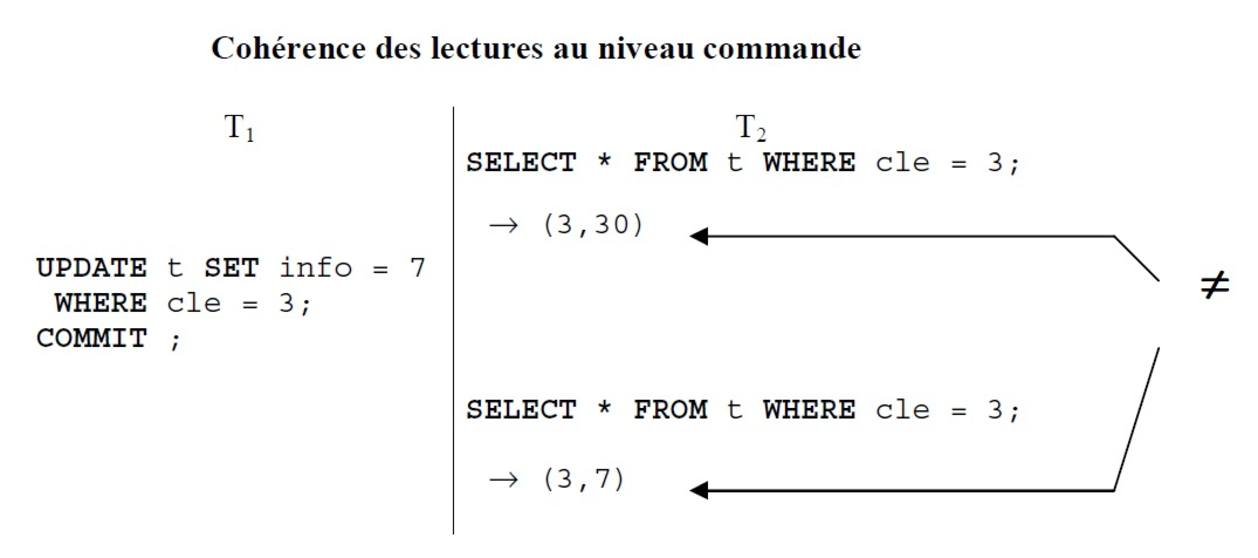
\includegraphics[width=0.85\textwidth]{../assets/img/coherence-de-lecture.pdf}
            \caption{Lecture non reproductible : niveau par défaut en Oracle.}
        \end{center}
    \end{figure}
\end{frame}

\begin{frame}{\secname : \subsecname}
    En Oracle : \textbf{une lecture ne bloque pas une modification et une modification ne bloque pas une lecture.}
    \begin{itemize}
        \item Si une transaction T2 tente de lire un objet sur lequel une transaction T1 possède un accès en écriture, alors T2 a accès à une version antérieurement confirmée de l'objet;
        \item Si une transaction T2 cherche à modifier un objet sur lequel une transaction T1 possède un accès en lecture, la transaction T2 obtient l'accès en écriture alors que T1 mémorise l'accès à sa version de l'objet (qui devient l'ancienne valeur dans le journal des images avant).
    \end{itemize}
\end{frame}

\begin{frame}{\secname : \subsecname}
    Comportements des accès concurrents par défaut
    \begin{itemize}
        \item Cette technique n'est utilisable que si le SGBD est capable de mémoriser une version antérieure confirmée.
        \item Rappel : par défaut, en Oracle, les lectures ne sont pas reproductibles (voir exemple ci-après).
    \end{itemize}
\end{frame}

\begin{frame}{\secname : \subsecname}
    \begin{figure}
        \begin{center}
            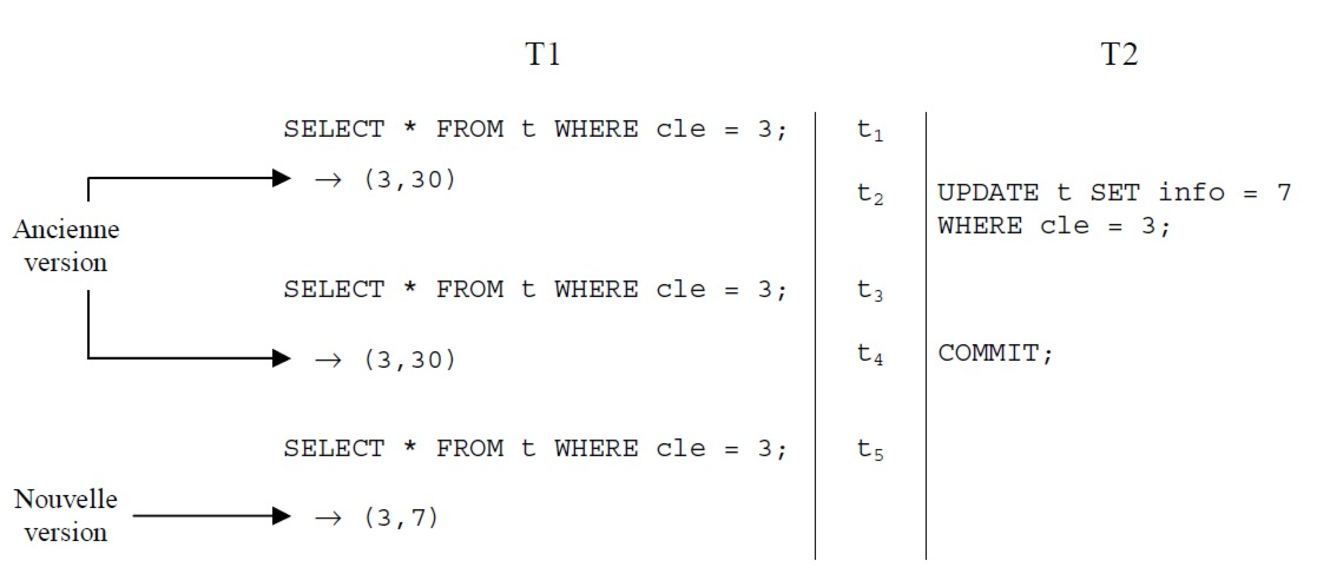
\includegraphics[width=\textwidth]{../assets/img/coherence-de-lecture-2.pdf}
            \caption{Comportements des accès concurrents par défaut}
        \end{center}
    \end{figure}
\end{frame}


\begin{frame}{\secname : \subsecname}
    Comportements des accès concurrents par défaut \\
    En Oracle : \textbf{une écriture bloque une écriture}.
\end{frame}

\begin{frame}{\secname : \subsecname}
    \begin{figure}
        \begin{center}
            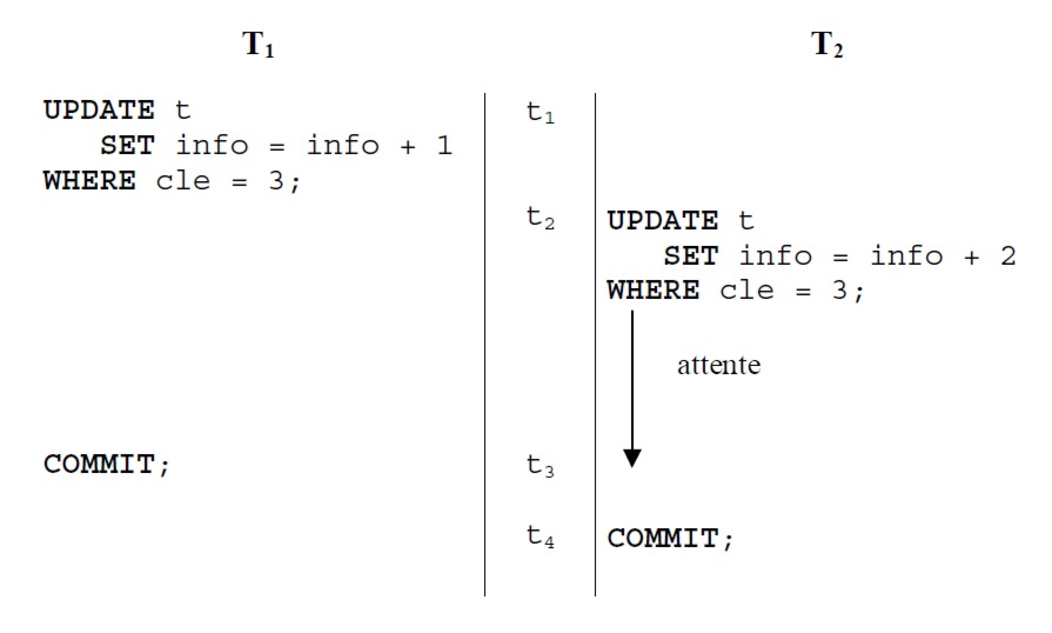
\includegraphics[width=\textwidth]{../assets/img/coherence-de-lecture-3.pdf}
            \caption{Dès que l'on commence un update, on a un verrou long, jusqu'à la fin de la transaction : COMMIT}
        \end{center}
    \end{figure}
\end{frame}

\begin{frame}{\secname : \subsecname}
    Comportements des accès concurrents par défaut \\
    En résumé, dans Oracle, lorsque l'on travaille avec les options par défaut :
    \begin{itemize}
        \pro Il n'y a pas de lecture impropre
        \pro Il n'y a pas de pertes de mises à jour
        \con Il est possible de provoquer une référence fantôme
        \con Les lectures ne sont pas forcément reproductibles
    \end{itemize}
\end{frame}

\begin{frame}{\secname : \subsecname}
    Oracle et les niveaux d'isolation
    \begin{itemize}
        \item Oracle empêche toute lecture impropre.
        \item Le niveau \lstinline[language=plsql]!READ COMMITTED! est le niveau par défaut.
        \item Oracle ne supporte pas directement le niveau \lstinline[language=plsql]!REPEATABLE READ! (il ne le supporte qu'on mode \lstinline[language=plsql]!READ ONLY!)
        \item En écriture, ce niveau est inclus dans le niveau \lstinline[language=plsql]!SERIALIZABLE!.
        \item Le niveau d'isolation est spécifié au moyen de la clause \lstinline[language=plsql]!ISOLATION LEVEL! de la commande \lstinline[language=plsql]!SET TRANSACTION!
    \end{itemize}
\end{frame}

\begin{frame}{\secname : \subsecname}
    \begin{figure}
        \begin{center}
            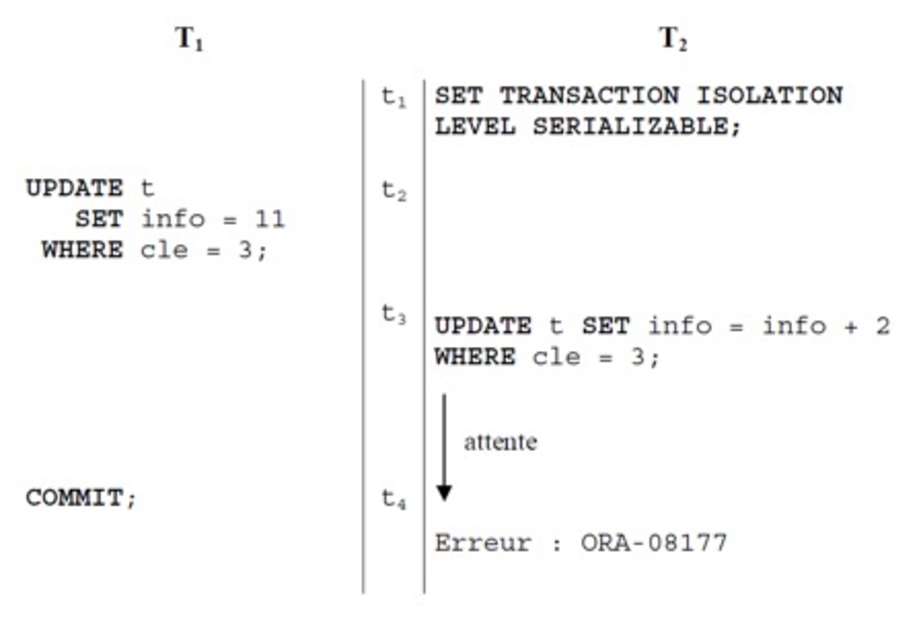
\includegraphics[width=0.9\textwidth]{../assets/img/coherence-de-lecture-4.pdf}
            \caption{Oracle et les niveaux d'isolation}
        \end{center}
    \end{figure}
\end{frame}
\begin{frame}{\secname : \subsecname}
    \begin{itemize}
        \item \textbf{t2}, T1 modifie le tuple 3, entraînant la pose d'un verrou en écriture sur ce tuple.
        \item \textbf{t3}, T2 veut, à son tour, modifier ce même tuple, T2 est placée en attente.
        \item \textbf{t4}, la transaction T1 libère les verrous et T2 est donc débloquée. Mais, à ce moment, T2 reçoit le code d'erreur ora-081177 indiquant qu'Oracle a détecté des données modifiées par une autre transaction depuis le début de la transaction sérialisable T2.
    \end{itemize}
\end{frame}
\subsection{Verrouillage explicite}
\begin{frame}{\secname : \subsecname}
    \begin{itemize}
        \item \textbf{t2}, T1 modifie le tuple 3, entraînant la pose d'un verrou en écriture sur ce tuple.
        \item \textbf{t3}, T2 veut, à son tour, modifier ce même tuple, T2 est placée en attente.
        \item \textbf{t4}, la transaction T1 libère les verrous et T2 est donc débloquée. Mais, à ce moment, T2 reçoit le code d'erreur ora-081177 indiquant qu'Oracle a détecté des données modifiées par une autre transaction depuis le début de la transaction sérialisable T2.
    \end{itemize}
\end{frame}

\begin{frame}{\secname : \subsecname}
    Oracle permet au programmeur de placer des verrous explicitement. Ceci se fait au moyen des commandes :
    \begin{itemize}
        \item \lstinline[language=plsql]!SELECT name FOR UPDATE [NOWAIT]!
        \item \lstinline[language=plsql]!LOCK TABLE!
    \end{itemize}
\end{frame}

\begin{frame}{\secname : \subsecname}
    \lstinputlisting[language=plsql, title=Verrouillage explicite dans Oracle]{../exemples/Chapitre 5/select-for-update.sql}
    Cette commande verrouille explicitement les tuples répondant à la condition de la clause \lstinline[language=plsql]!WHERE!.
    \lstinline[language=plsql]!verrou ROW SHARE!
    Les tuples sont verrouillés en vue d'être modifiés.  Une autre transaction pourra lire ces tuples mais pas les modifier.
\end{frame}

\begin{frame}{\secname : \subsecname}
    \lstinputlisting[language=plsql, title=Ici on ne souhaite pas attendre et donc risque d'erreur]{../exemples/Chapitre 5/select-for-update2.sql}
\end{frame}

\subsection{La double transaction}
\begin{frame}{\secname : \subsecname}
    \begin{itemize}
        \item  La double transaction va être mise en place dans le cadre de la mise à jour de données de la base lorsque plusieurs utilisateurs sont susceptibles de modifier les mêmes tuples.
        \item Les programmes qui la mettent en œuvre utilisent deux transactions d'où son nom.
              \begin{itemize}
                  \item première transaction : recherche du tuple à modifier
                  \item deuxième transaction : mise à jour des données
              \end{itemize}
        \item Entre les deux :
              \begin{itemize}
                  \item L'utilisateur courant peut faire des modifications (dans sa copie locale du tuple)
                  \item D'autres utilisateurs peuvent faire des mises à jour incompatibles
              \end{itemize}
    \end{itemize}
\end{frame}

\begin{frame}{\secname : \subsecname}
    Exemple :  Un étudiant a changé d'adresse et va au service étudiant pour le faire savoir.
    \begin{itemize}
        \item Lecture de la donnée à modifier (recherche de l'étudiant à modifier)
        \item Encodage de la nouvelle valeur
        \item Mise à jour de cette valeur
    \end{itemize}
\end{frame}

\begin{frame}{\secname : \subsecname}
    \begin{itemize}
        \item  Si on est tout seul à travailler sur la BD, pas de soucis
        \item S'il y a plusieurs utilisateurs susceptibles d'apporter des modifications aux données de la base, on peut lire la donnée à modifier en posant un verrou, on encode la nouvelle valeur, on met à jour et on libère le verrou.
        \item Le problème peut apparaître au niveau de l'encodage de la nouvelle valeur -> phénomène de la tasse de café
    \end{itemize}
\end{frame}

\begin{frame}{\secname : \subsecname}
    \begin{itemize}
        \item  Lire le tuple à modifier (ancien tuple) et la lecture sera faite sans verrou !
        \item Encoder les nouvelles valeurs : nouveau tuple
        \item Relire le tuple à modifer en posant un verrou avec l'option \lstinline[language=plsql]!NOWAIT! dans l'idée de le remplacer par le tuple qui contient les nouvelles valeurs.
    \end{itemize}
\end{frame}

\begin{frame}{\secname : \subsecname}
    Trois cas de figure peuvent se présenter lors de la lecture du tuple avec pose de verrou :
    \begin{itemize}
        \item La ressource est occupée (-54)
        \item La ressource n'existe plus (\lstinline[language=plsql]!NO\_DATA\_FOUND!)
        \item La ressource est disponible.
    \end{itemize}
\end{frame}

\begin{frame}{\secname : \subsecname}
    \textbf{La ressource est occupée (-54)}
    Dans ce cas, on peut choisir d'attendre un moment et de refaire une tentative quelques instants plus tard.
    Si tout utilisateur qui accède à la BD le fait de manière correcte, la ressource ne devrait pas être bloquée longtemps.
    On peut répéter la séquence tentative/attente plusieurs fois (souvent on se limite à 3), si la ressource est toujours bloquée on abandonne la modification.
\end{frame}

\begin{frame}{\secname : \subsecname}
    \textbf{La ressource n'existe plus (\lstinline[language=plsql]!NO\_DATA\_FOUND!)}
    La ressource a été supprimée entretemps, la modification est alors interrompue
\end{frame}
\begin{frame}{\secname : \subsecname}
    \textbf{La ressource est disponible}
    Il faut vérifier qu'elle n'a pas été modifiée entretemps par un autre utilisateur
    On va alors comparer l'ancien tuple à celui que l'on vient de lire.  La comparaison se fait champ par champ.
    Si les 2 tuples sont identiques, on va pouvoir insérer le tuple modifié et valider
    S'ils sont différents, le tuple a été modifié entretemps par un autre utilisateur, la modification courante est alors abandonnée.  Ne pas oublier de libérer le verrou.
\end{frame}

\end{document}